\documentclass[8pt]{beamer}

\usepackage[utf8]{inputenc}       % mit fontenc: Umlaute und ß (sz) direkt eingeben
\usepackage[T1]{fontenc}          % ^...^

\usepackage{libertine}
\usepackage{color}
\usepackage{graphicx}

\usepackage{booktabs}             % table decorations

\usepackage{amsmath}
\usepackage{amssymb}
\usepackage{mathrsfs}             % calligraphie

\usepackage{siunitx}
\newcommand\unit[2]{\SI{#1}{#2}}

% \usepackage{feynmf}%%%{feynmp}    % Feynman Diagramme
% \unitlength=1mm

% \usepackage[percent]{overpic}     % draw text atop of pictures

\usepackage{tikz}                 % drawing shapes
\usetikzlibrary{plotmarks,patterns,calc,decorations.markings,arrows,intersections,decorations.pathmorphing}
\tikzset{snake it/.style={decorate, decoration=snake}}

\usepackage{pgfplots}
\usepgflibrary{shapes}
\usepgfplotslibrary{groupplots}
\pgfplotsset{compat=newest}
\newlength{\figurewidth}
\setlength{\figurewidth}{6cm}
\newlength{\figureheight}
\setlength{\figureheight}{5cm}

% \usepackage{pgffor}               % for-loop

% \usepackage{pdfpages}






\usetheme{Warsaw}
\useoutertheme{infolines}

\usecolortheme{rose}                            % invertiert fg/bg von block-titeln
\usecolortheme{beaver}                          % helles, rotes outercolortheme
\usecolortheme[rgb={0.5,0,0}]{structure}        % setzt innere fg color auf dunkelrot
\beamertemplatenavigationsymbolsempty



\def\Put(#1,#2)#3{\leavevmode\makebox(0,0){\put(#1,#2){#3}}}


\def\mydate{\leavevmode\hbox{\the\year-\twodigits\month-20}}
\def\twodigits#1{\ifnum#1<10 0\fi\the#1}


\title{to recap my workflow}
\subtitle{}
\author[Tino Michael]{Tino Michael\vspace{-12pt}}
\institute[CEA Saclay]{CEA Saclay, Irfu/SAp}
% \institute[CEA]{Commissariat à l'énergie atomique et aux énergies alternatives}
\titlegraphic{
    \begin{tikzpicture}
        \node (centre) at (0,0)                       {\includegraphics[height=40pt]{../Resources/Pictures/Logo_CEA_2012.png}};
        \node[anchor=west] at ([xshift=-150pt]centre) {\includegraphics[height=40pt]{../Resources/Pictures/Logo_Asterics.png}};
        \node[anchor=east] at ([xshift=+150pt]centre) {\includegraphics[height=40pt]{../Resources/Pictures/Logo_CTA_blue.png}};
    \end{tikzpicture}
}
\date[\mydate]{Group Meeting\\\mydate}



\begin{document}

    \definecolor{darkred}{rgb}{0.5,0,0}
    \setbeamertemplate{section in toc}[circle]
    \setbeamerfont{section number projected}{%
        family=\rmfamily,series=\bfseries,size=\normalsize}
    \setbeamercolor{section number projected}{bg=white,fg=darkred}

    \begin{frame}
        \titlepage
    \end{frame}



    \begin{frame}{Shower Reconstruction}
        \begin{columns}
            \column{.6\textwidth}
                \begin{tikzpicture}
                \only<1>{
                    \node[anchor = center] (pic1) at (0,0) {
                        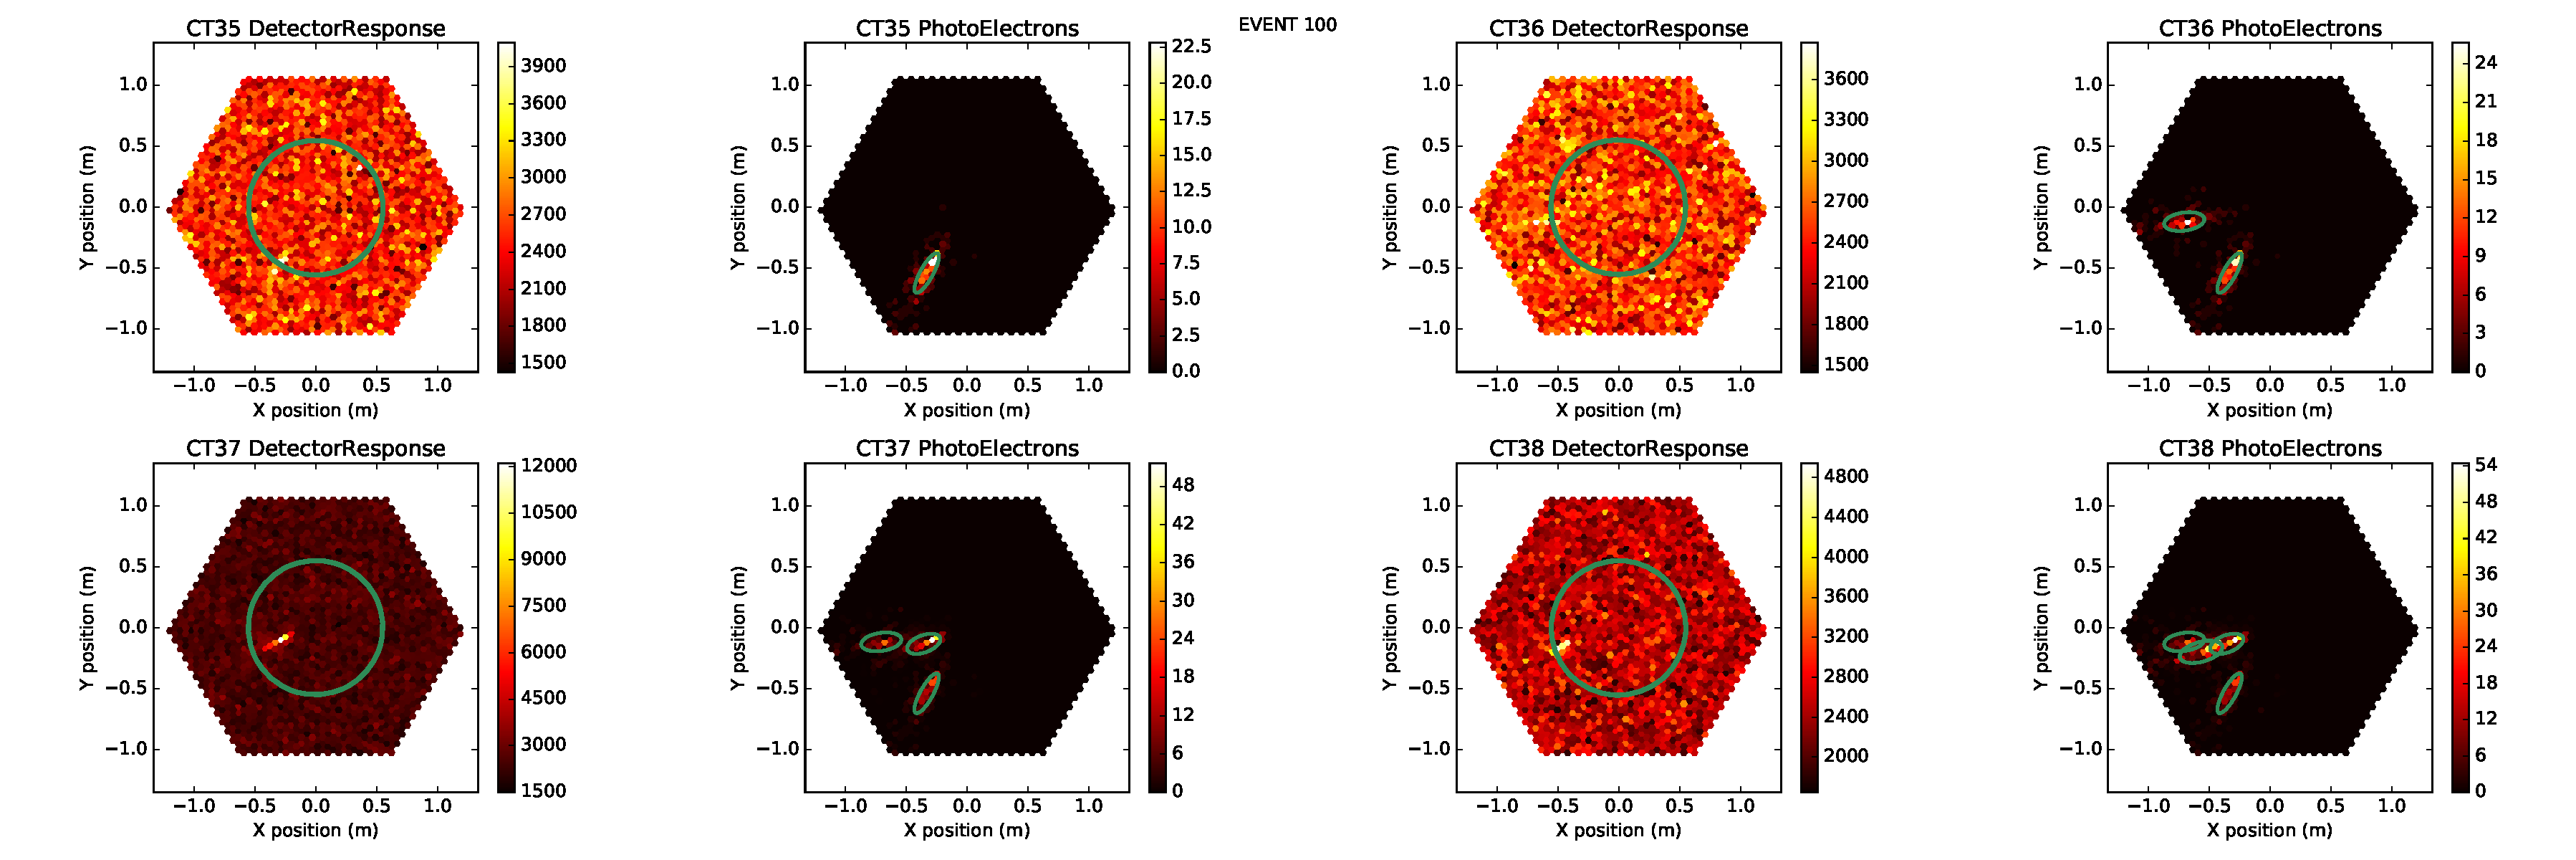
\includegraphics[trim=17cm 10cm 32cm .85cm,clip,
                                                width=\textwidth]{pics/hillas_overlay}
                    };
                }
                \only<2->{
                    \node[anchor = center] (pic1) at (0,0) {
                        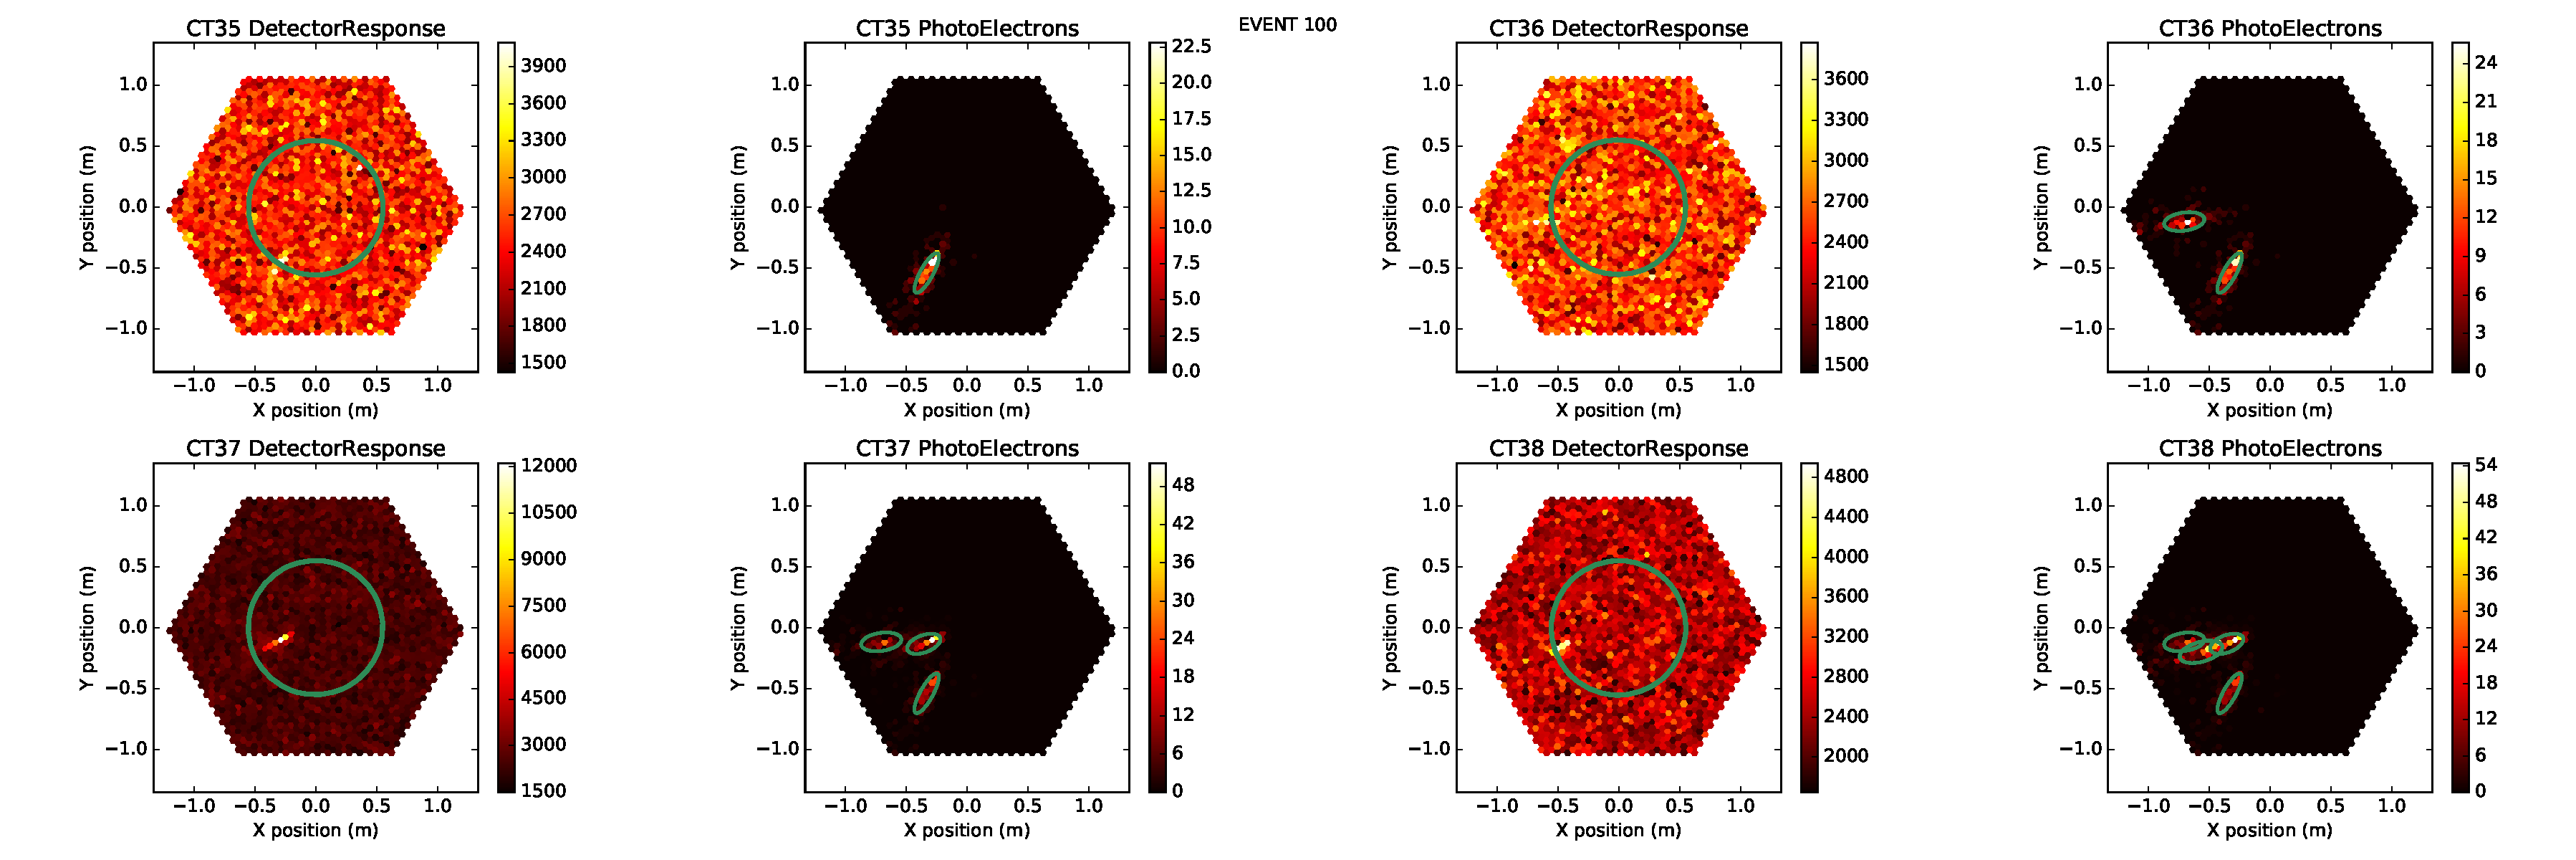
\includegraphics[trim=17cm .2cm 32cm 10.85cm,clip,
                                                width=\textwidth]{pics/hillas_overlay}
                    };
                }
                \only<3->{
                    \draw[line width=.4mm,green] (0,5.8mm) -- +(240.5:2cm);
                    \draw[line width=.4mm,green] (0,4.2mm) -- +(200:2cm);
                    \draw[line width=.4mm,green] (0,3.9mm) -- +(188:2cm);
                }
                \end{tikzpicture}
            \column{.4\textwidth}
                \begin{itemize}
                    \item construct an ellipsis with moments of the shower image:\\
                    \emph{Hillas Parametrisation}
                    \pause
                    \item combine images from different cameras
                    \pause
                    \item intersection of their ellipsis axes is
                        the shower origin
                \end{itemize}

        \end{columns}

    \end{frame}



    \begin{frame}{Next Steps}
        \begin{columns}
            \column{.5\textwidth}

                \begin{itemize}
                    \item [] Photon / Proton Discrimination
                    \item Protons pose major background
                    \item Event rate about $10^5$ times above Photons
                    \item[]
                    \item[] H.E.S.S. methode:
                    \item reducing total signal on camera, length and width
                        of ellipsis and their variances from all telescopes
                        into one parameter to cut on
                    \item[]
                    \item[] here instead:
                    \item Discrimination with \emph{RandomForestClassifier}\\
                        fed with parameters from each camera image and the whole event
                \end{itemize}
            \column{.5\textwidth}
                \centering
                \begin{tikzpicture}
                    \node[anchor=south] (pic1) at (0,0)
                            {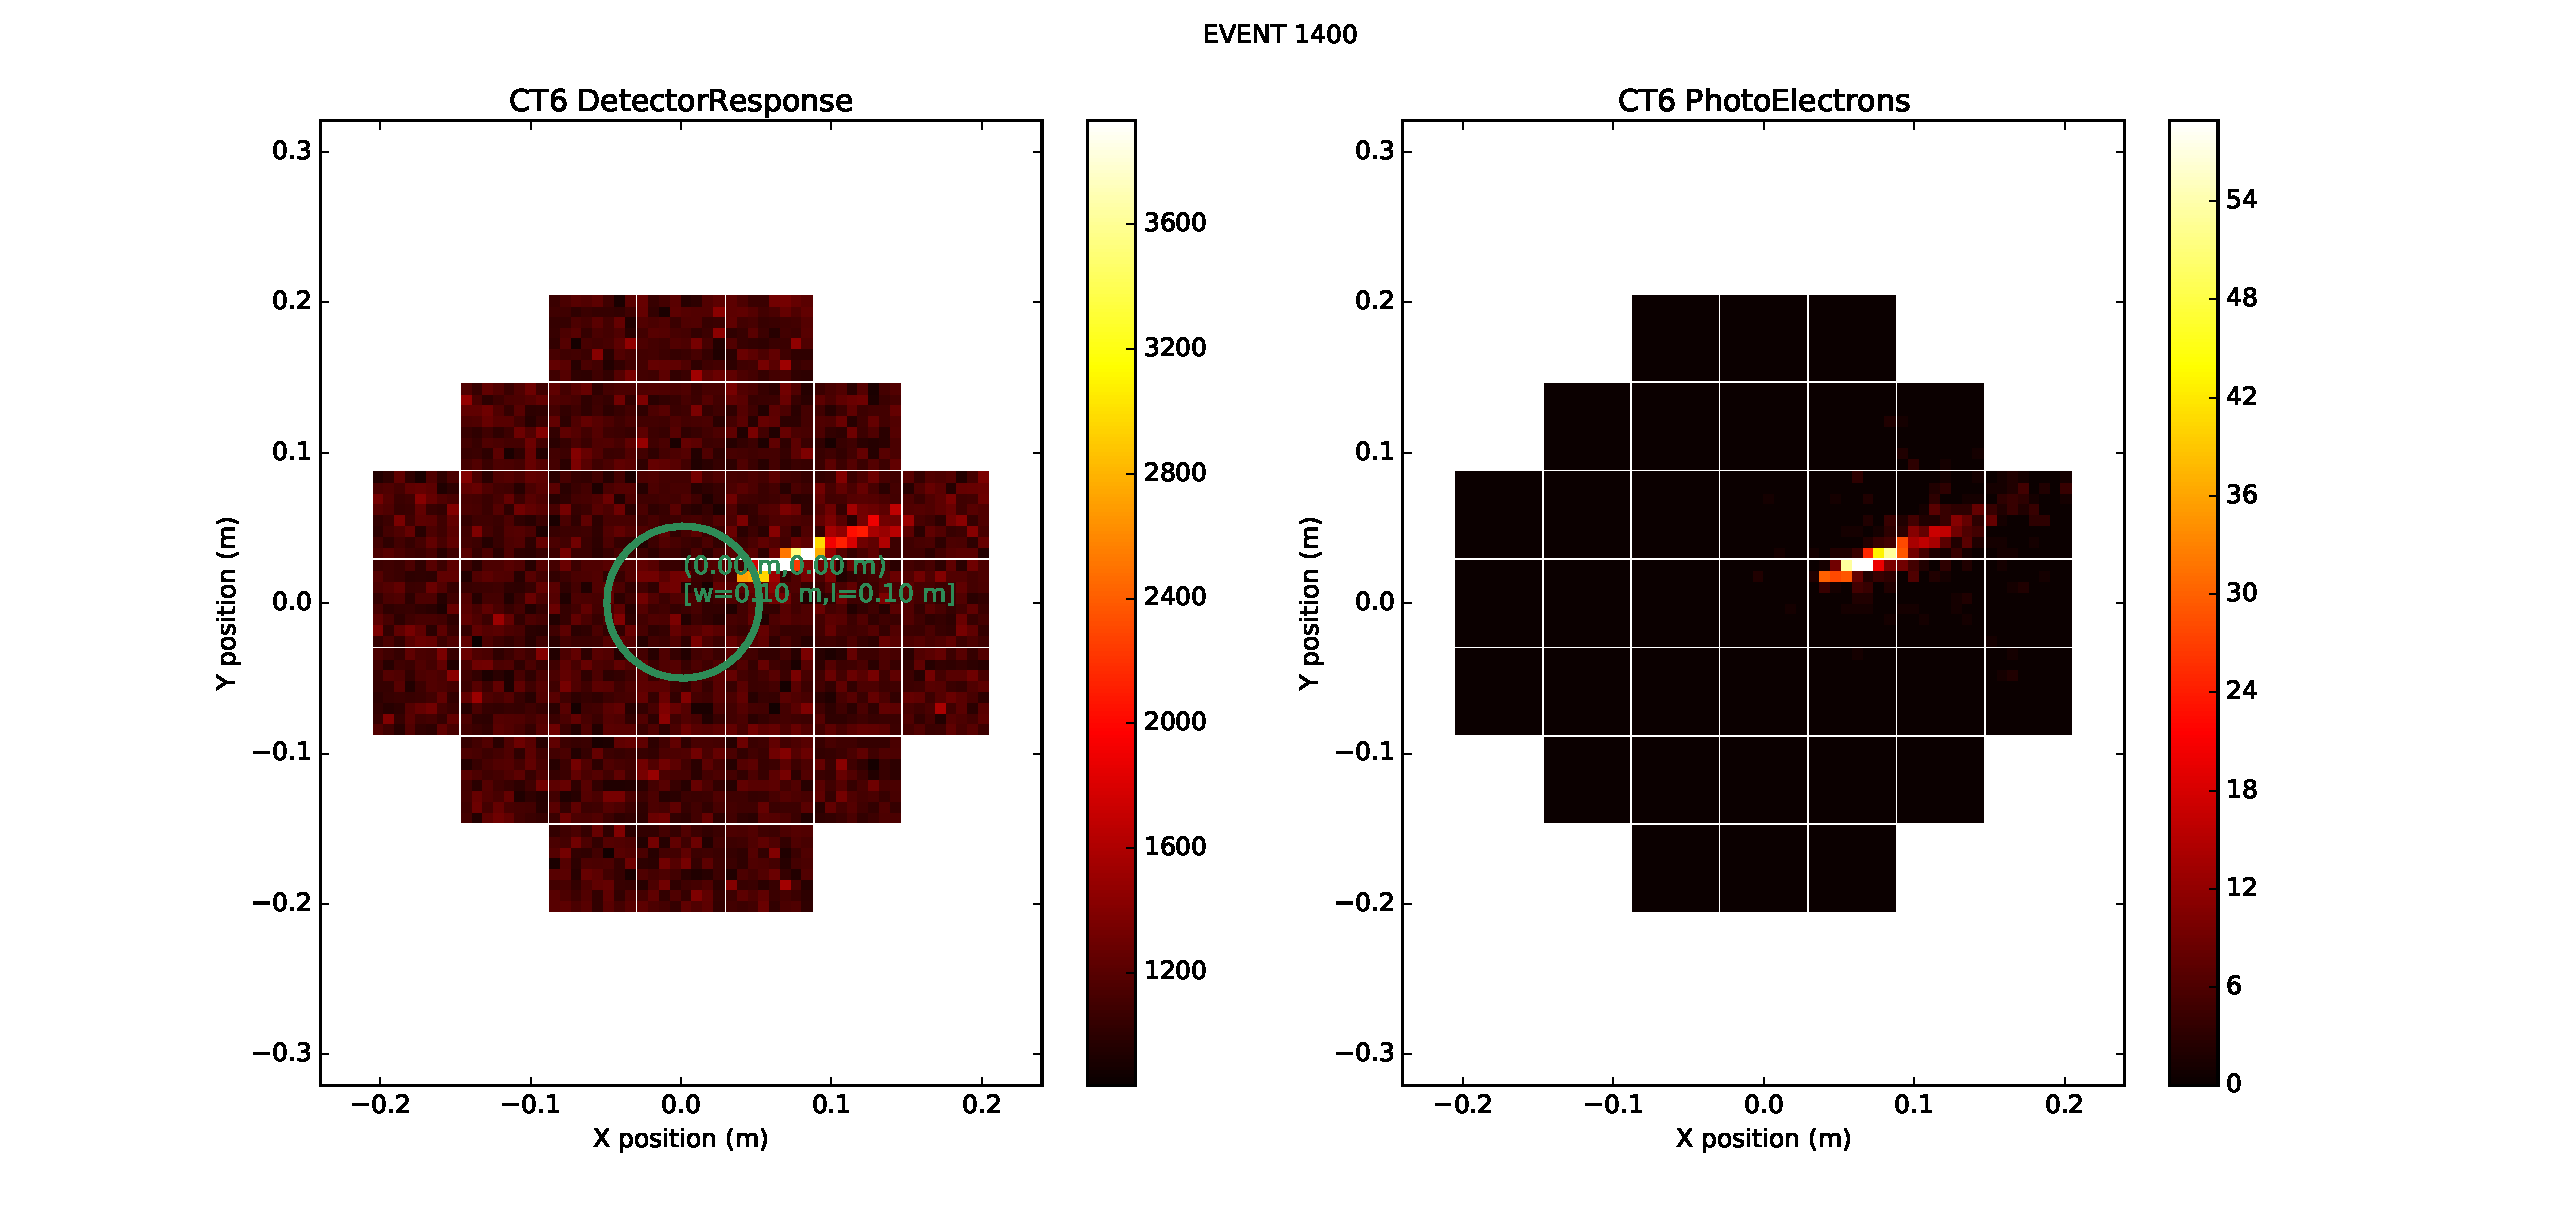
\includegraphics[trim=22cm 0 4cm 2cm,clip,width=.6\textwidth]
                                                                    {pics/photon_1}};
                    \node[anchor=north] (pic2) at (pic1.south)
                            {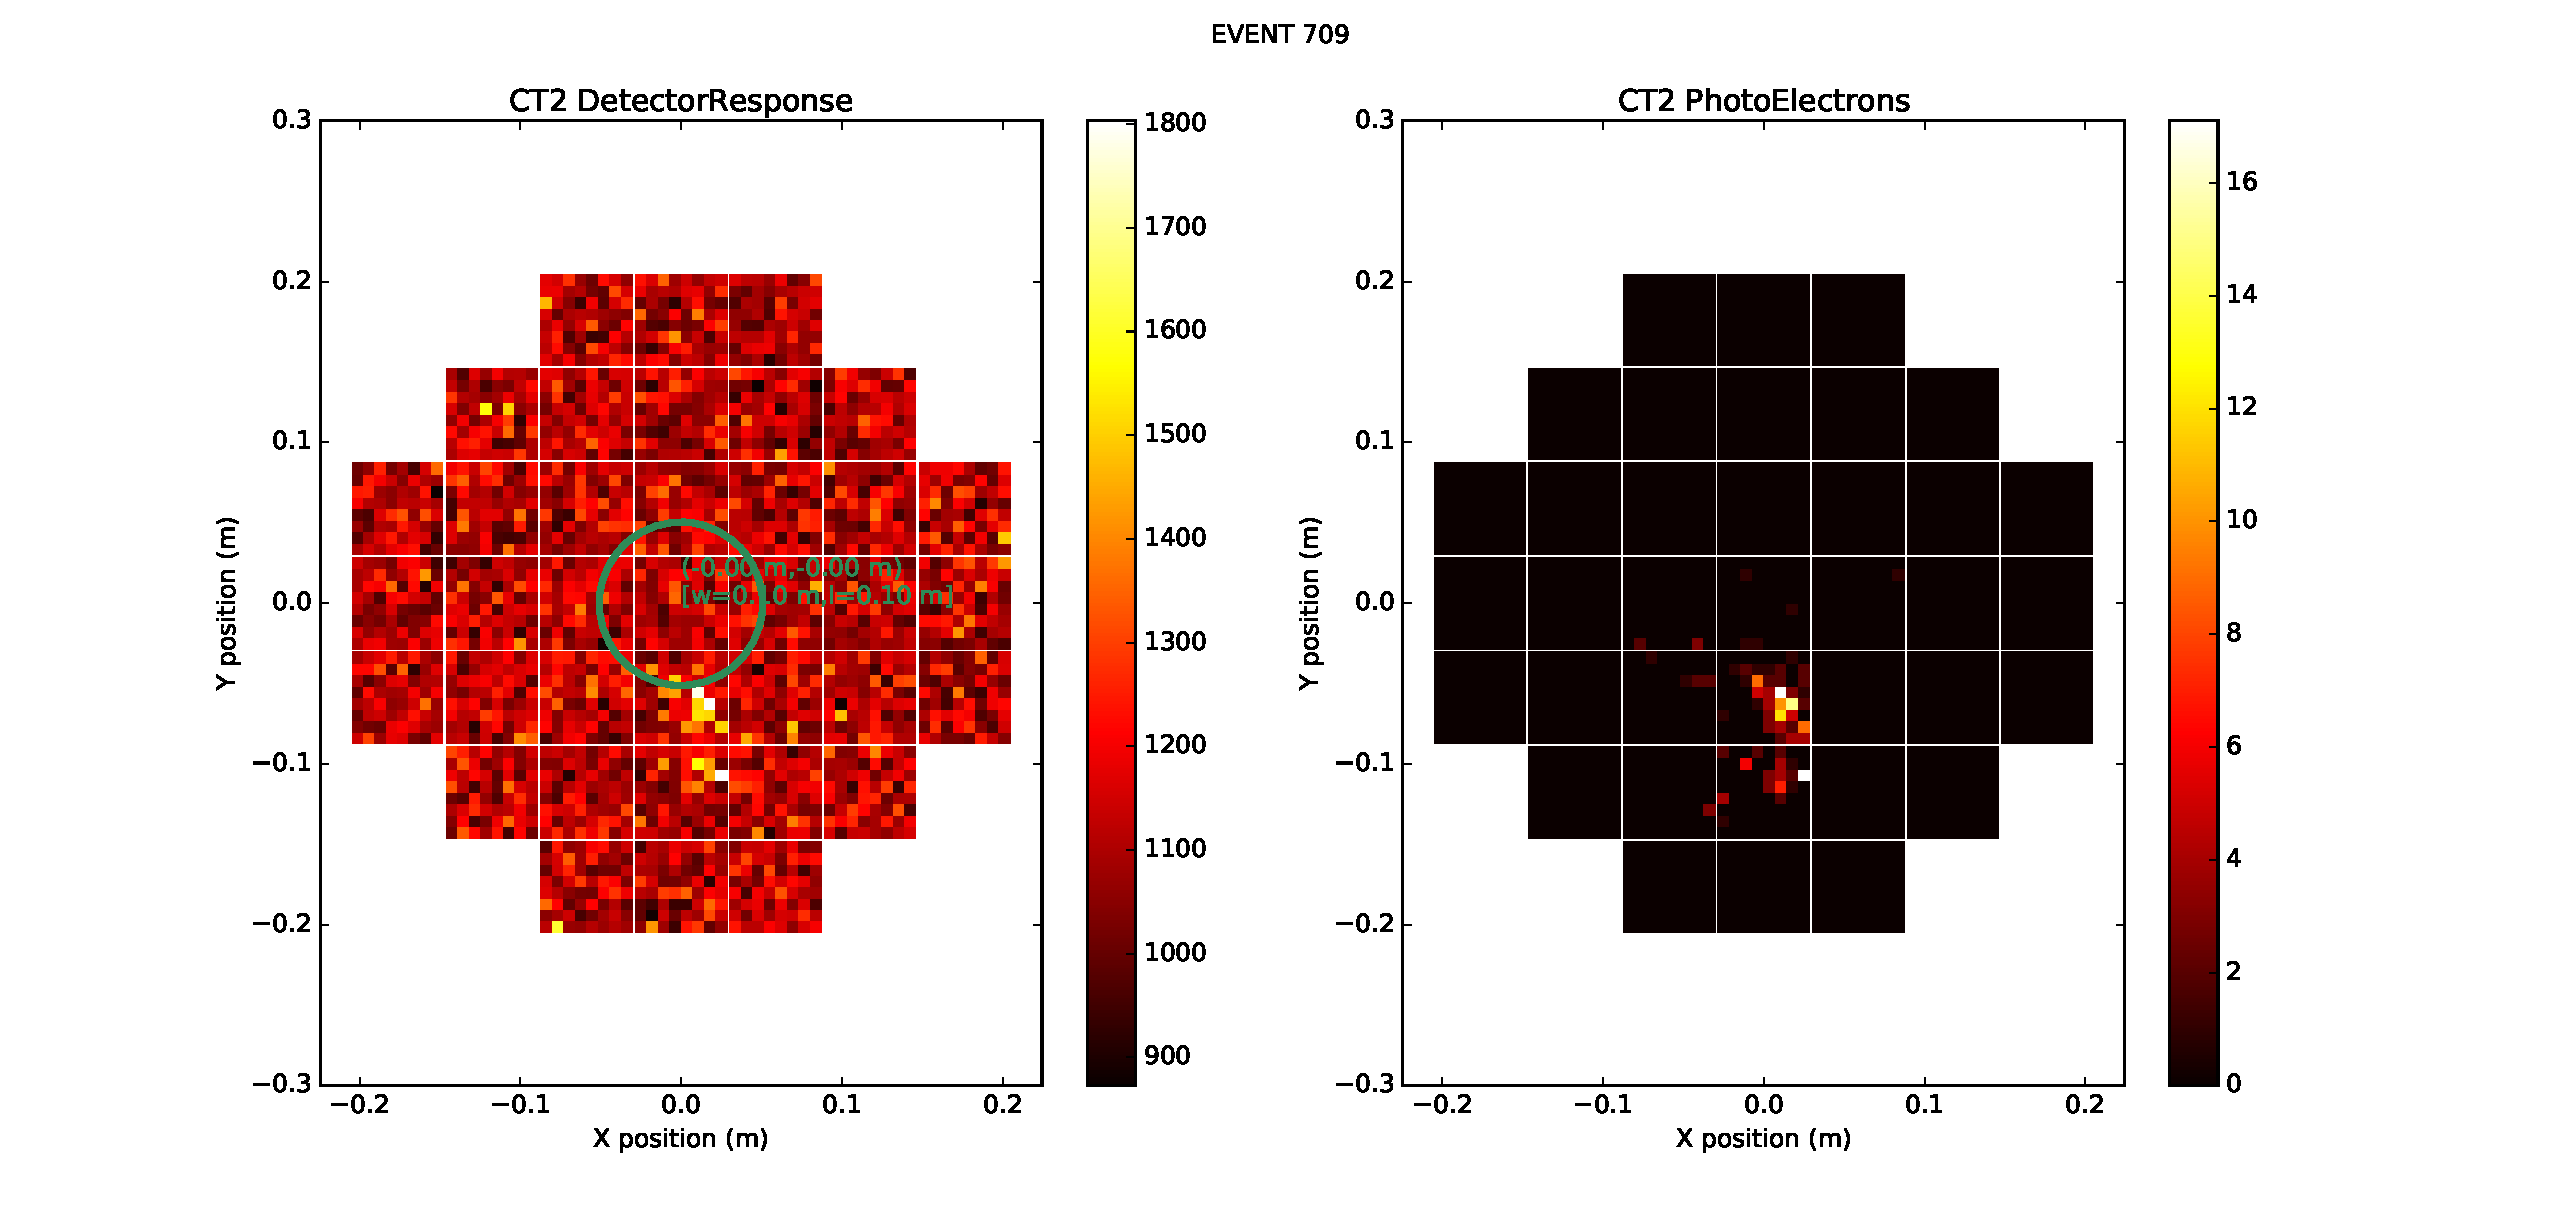
\includegraphics[trim=22cm 0 4cm 2cm,clip,width=.6\textwidth]
                                                                    {pics/proton_1}};
                    \node[anchor=south,rotate=90] at (pic1.west) {photon};
                    \node[anchor=south,rotate=90] at (pic2.west) {proton};
                \end{tikzpicture}
        \end{columns}
    \end{frame}

    \begin{frame}{Discrimination}

        \centering

        \begin{itemize}
            \item using RandomForestClassifier implemented in \emph{scikit-learn}
            \item data-mining approach: just throw all the data at it that we have
                \begin{itemize}
                    \item distance between telescope reconstructed impact position
                    \item error estimate on the impact position
                    \item Hillas parameters: width, length, skewness, kurtosis
                    \item total signal on camera
                    \item signal of the pixel with the highest count
                    \item total signal on all selected telescopes
                    \item number of selected telescopes
                \end{itemize}
        \end{itemize}

        \pause

        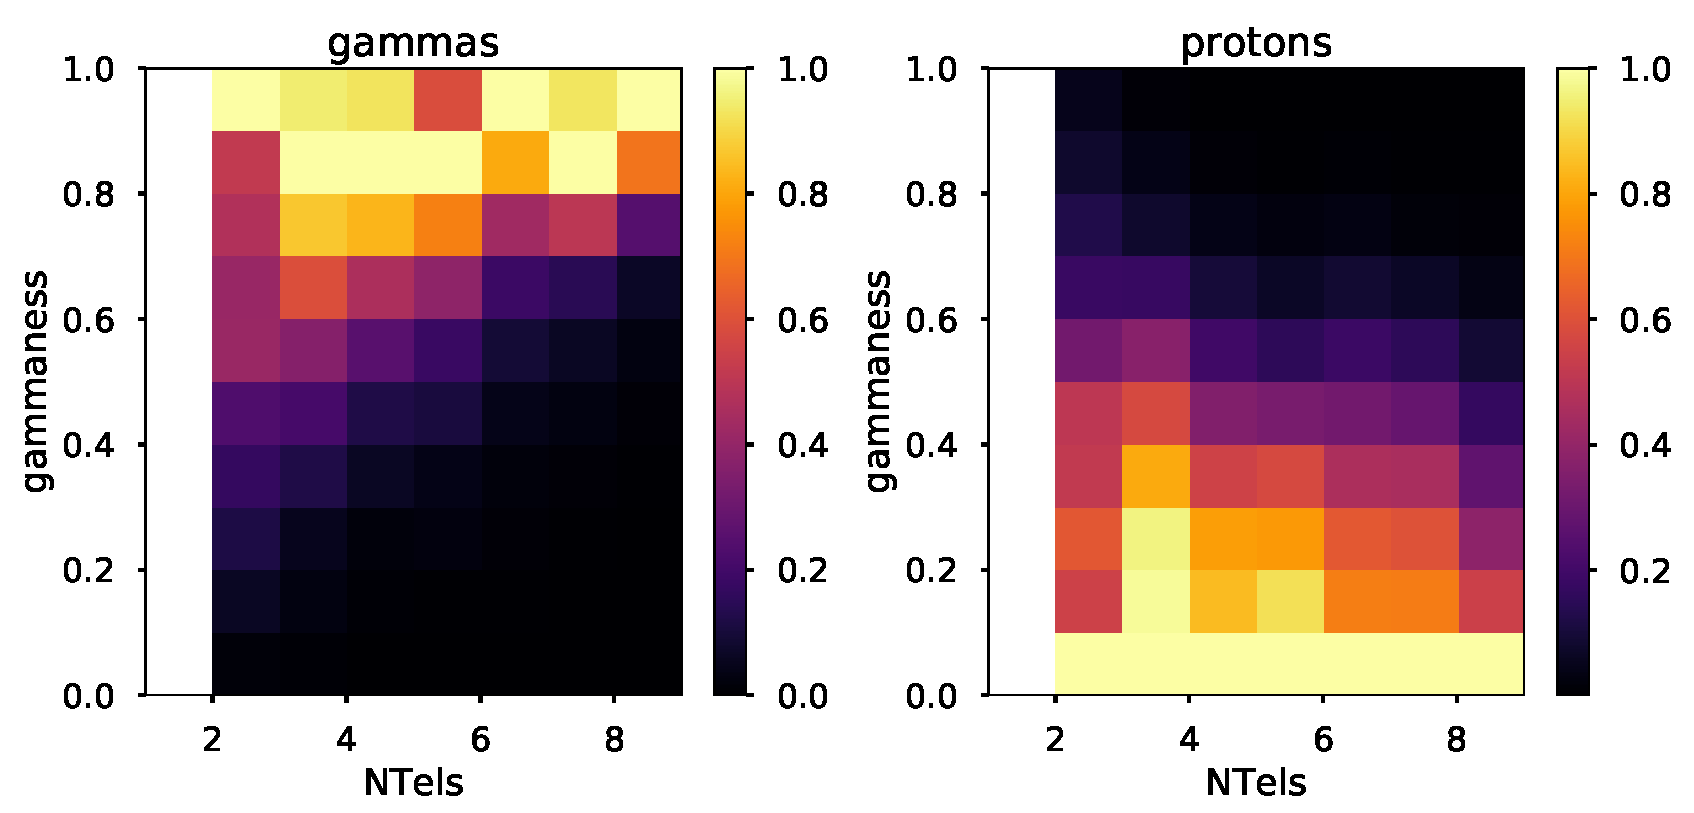
\includegraphics[width=.7\textwidth]{pics/gammaness_gamma_proton_tail}

        \pause

        for now, cut on $NTels > 2 \ \&\ gammaness > 0.75$
    \end{frame}


    \begin{frame}{generated and selected MC events}
        \centering
        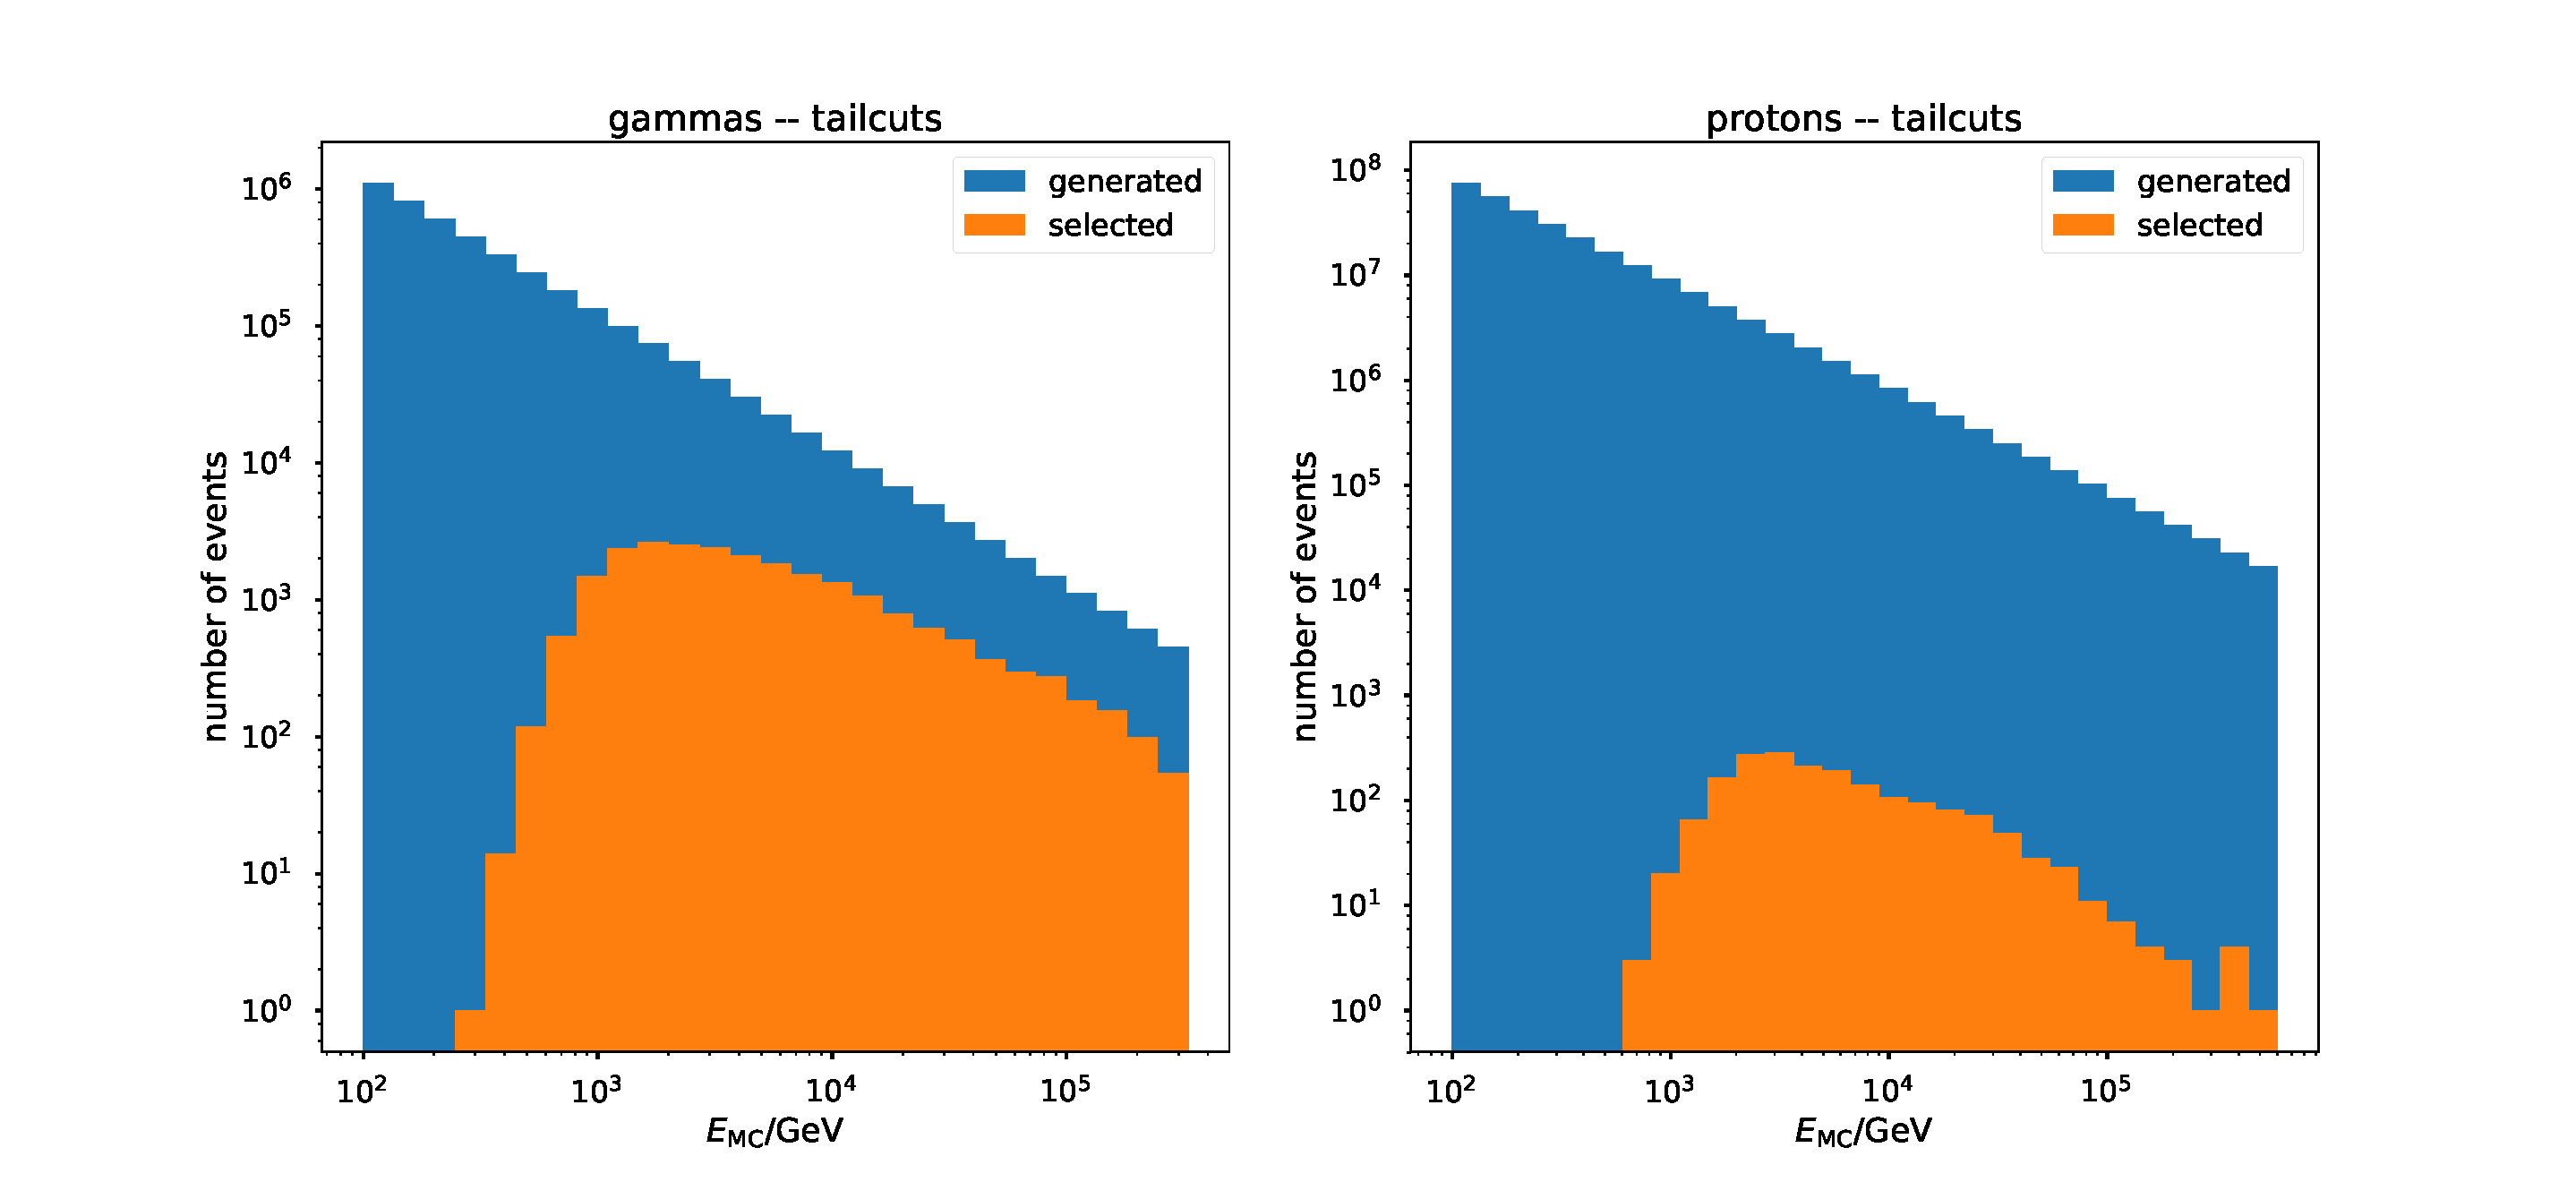
\includegraphics[trim=3cm 0 4cm 0,clip, width=1.\textwidth]
                                                            {pics/NEvents_vs_energy_MC}

    \end{frame}


    \begin{frame}{Effective Area}
        taking the ratio of the previous plots (i.e. the selection efficiency) and
        multiply every bin with the area in which the MC events have been generated in:
        \emph{Effective Area}\vspace{5mm}

        \centering
        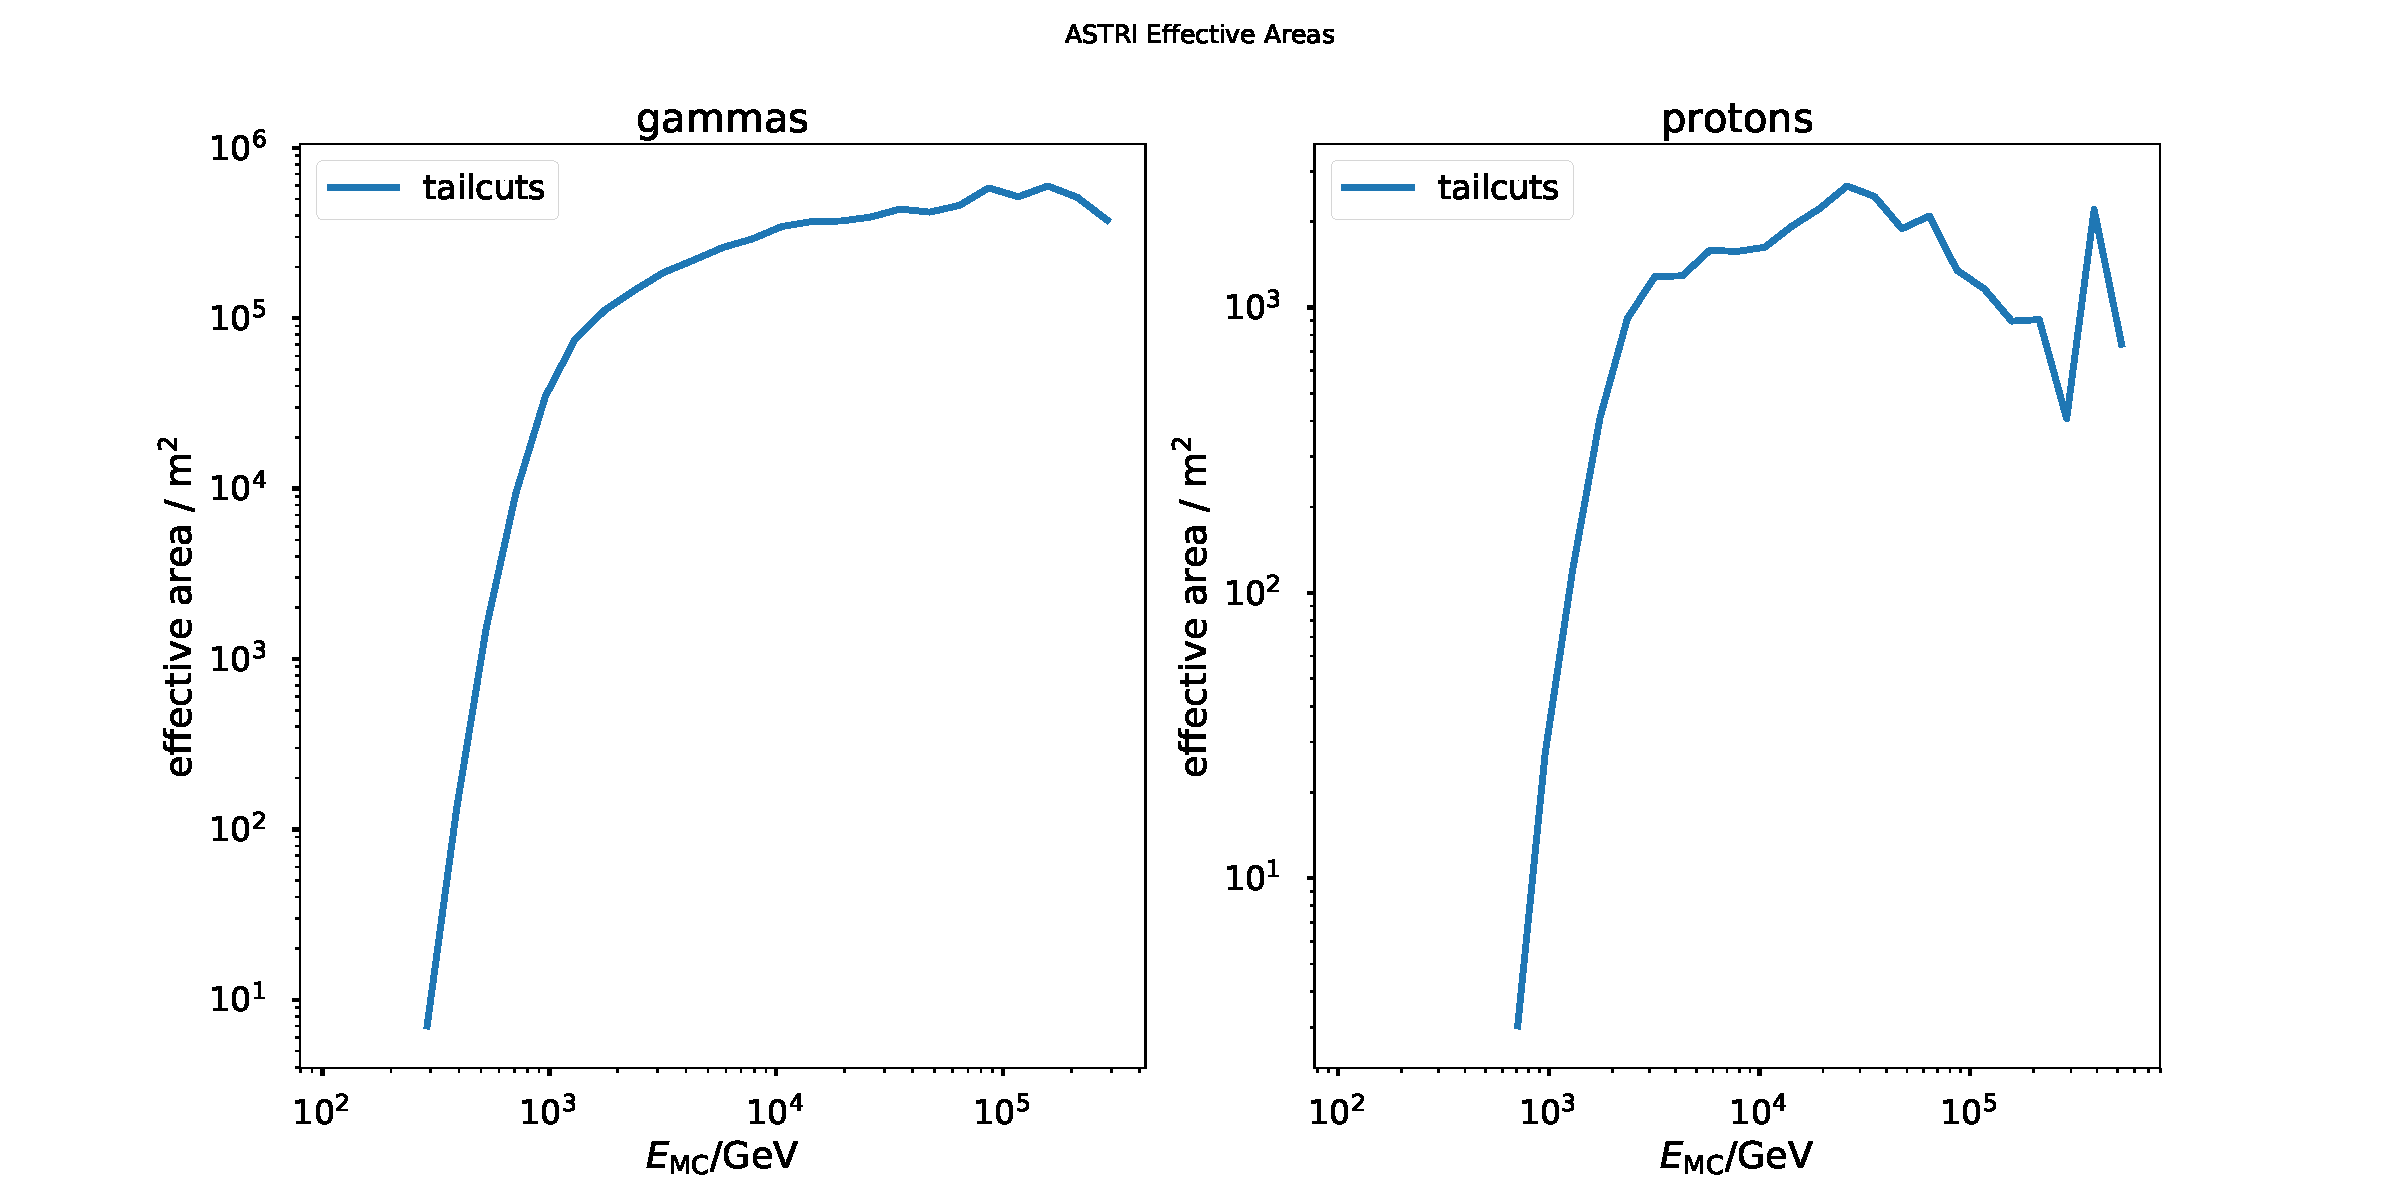
\includegraphics[trim=2cm 0 3cm 1cm, clip, width=\textwidth]{pics/effective_areas}

    \end{frame}


    \begin{frame}
        \begin{itemize}
            \item next step: reweighting of MC events to correspond to expected physical
                flux (e.g. Crab nebula)
            \only<2>{
                \item but how?
            }
            \only<3,4>{
                \item simple binned approach:
                    \begin{itemize}
                        \item already have the energy-binned efficiencies
                        \item apply these on the energy-binned histogram of expected
                            \emph{arriving} events from the source
                        \item \textrightarrow\ get the number of expected selected events
                    \end{itemize}
                \only<4>{
                    \item \textbf{but:} it's binned... not nice
                }
            }
            \only<5->{
                \item instead: event-by-event weight that considers the generator
                    spectrum:
                \item $w(E) = A_\mathrm{gen} \times I_\Theta \times E^\gamma \times I_E
                    \times T_\mathrm{obs}/ N_\mathrm{gen}$\\ with:
                    \begin{itemize}
                        \item $A_\mathrm{gen}$: MC generator Area
                        \item $I_\Theta = 2 \pi (1-\cos\vartheta)$: angular phase space
                            factor for diffuse flux
                        \item $E^\gamma$: considers that MC events have been drawn with an
                            $E^{-2}$ spectrum
                        \item $\gamma$: spectral index of the MC generator (here equal 2)
                        \item $I_E =
                            (E_\mathrm{max}^{(1-\gamma)} - E_\mathrm{min}^{(1-\gamma)})
                            / (1-\gamma)$: energy phase space factor
                        \item $T_\mathrm{obs}$: assumed observation time
                        \item $N_\mathrm{gen}$: number of generated MC events
                    \end{itemize}
                \item $w(E) \times \varPhi(E)$ gives weight for every MC event so that
                    their energy distribution looks like the selected events from the
                    assumed flux $\varPhi$

            }
            \pause\pause\pause\pause\pause
            \item described in old ANTARES internal note: ANTARES-SOFT-1999-003
        \end{itemize}

    \end{frame}


    \begin{frame}{Expected Events from Crab and Cosmic Rays}
        \centering
        \only<1>{
            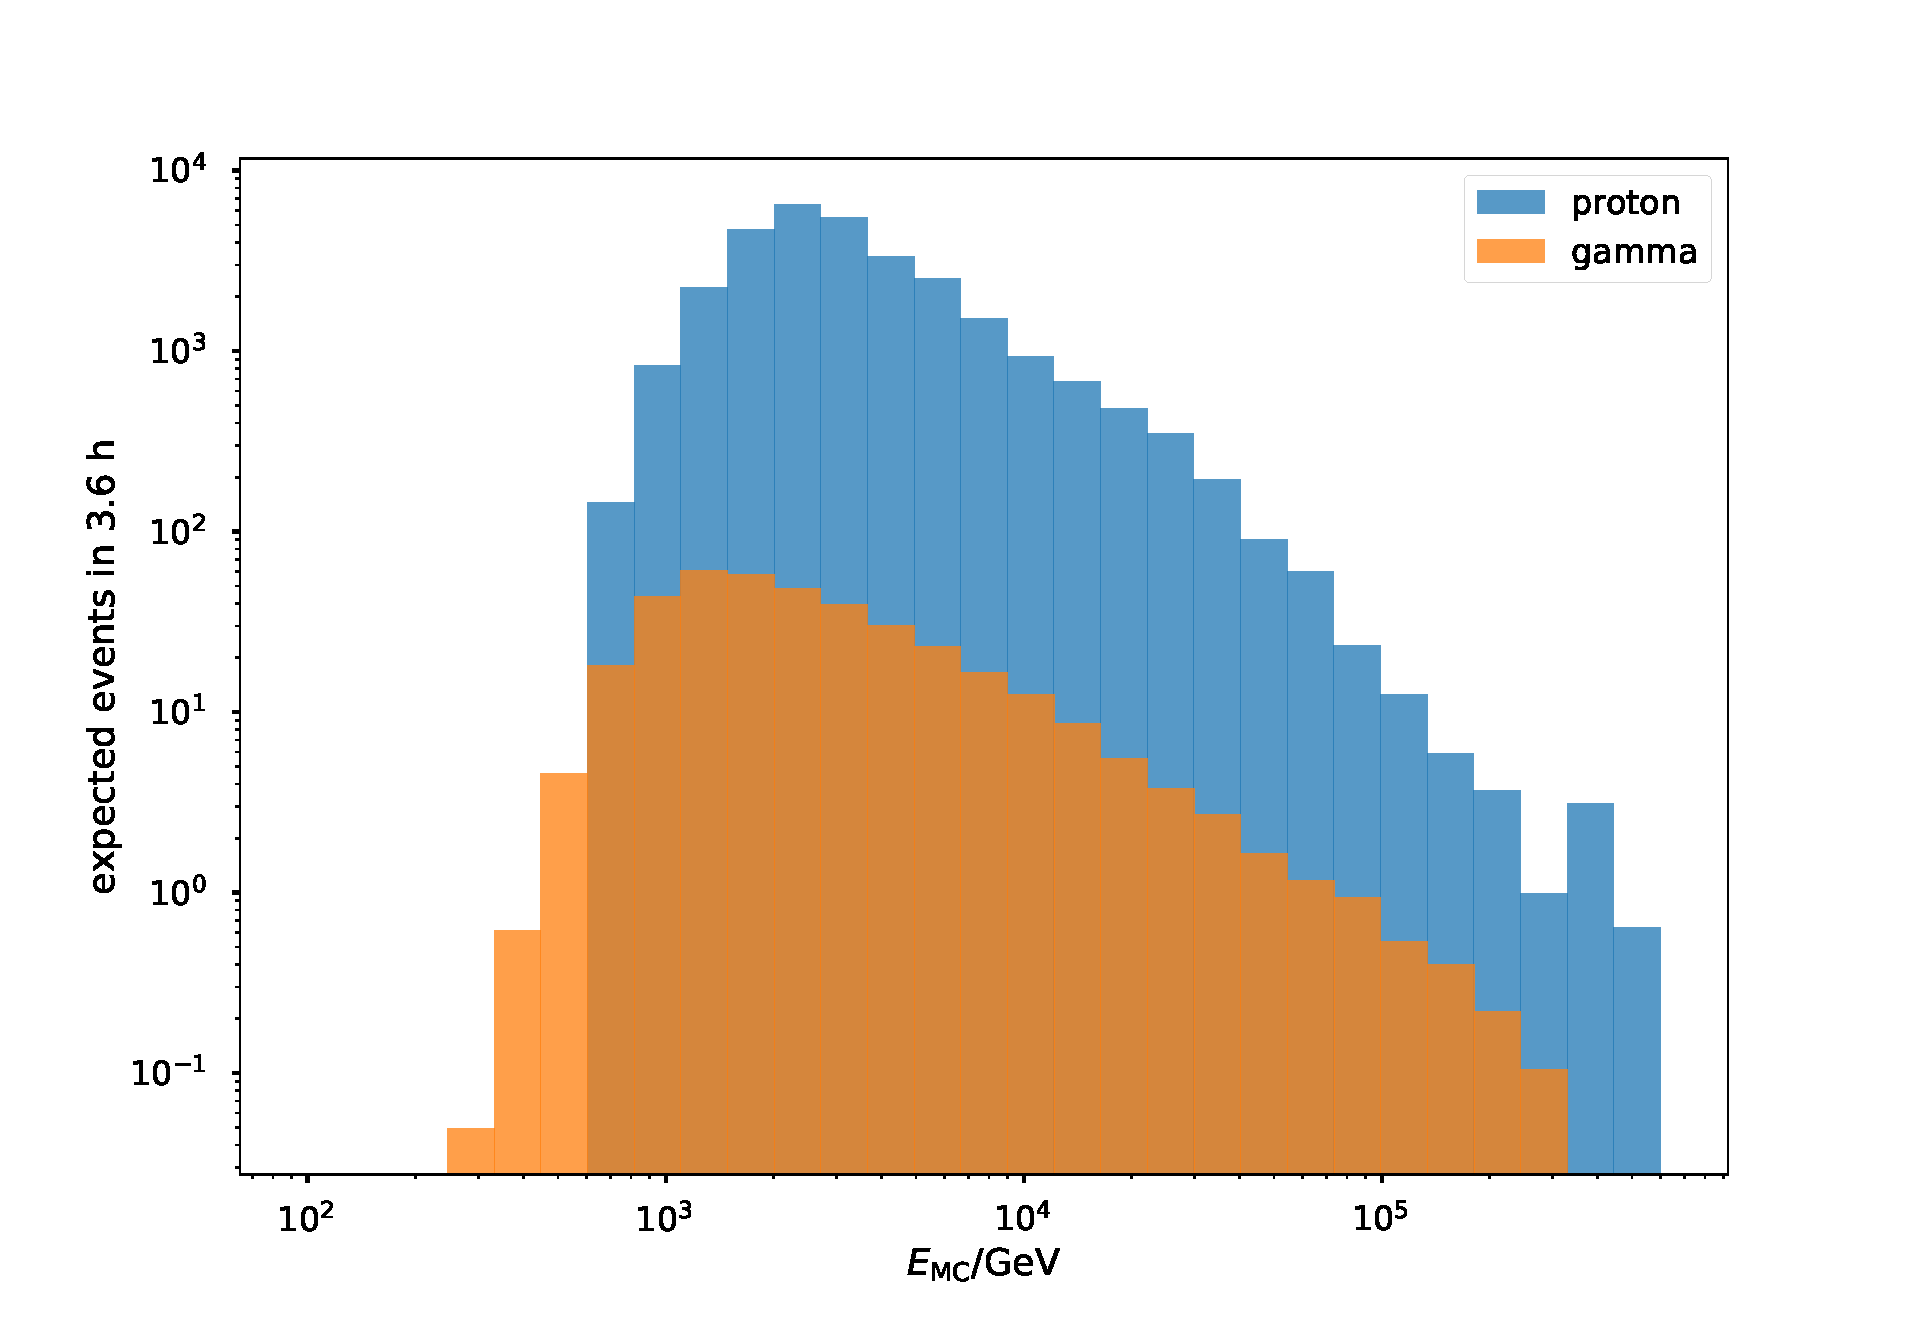
\includegraphics[width=\textwidth]{{pics/expected_events_3.6h_tail}.pdf}
        }
        \only<2>{
            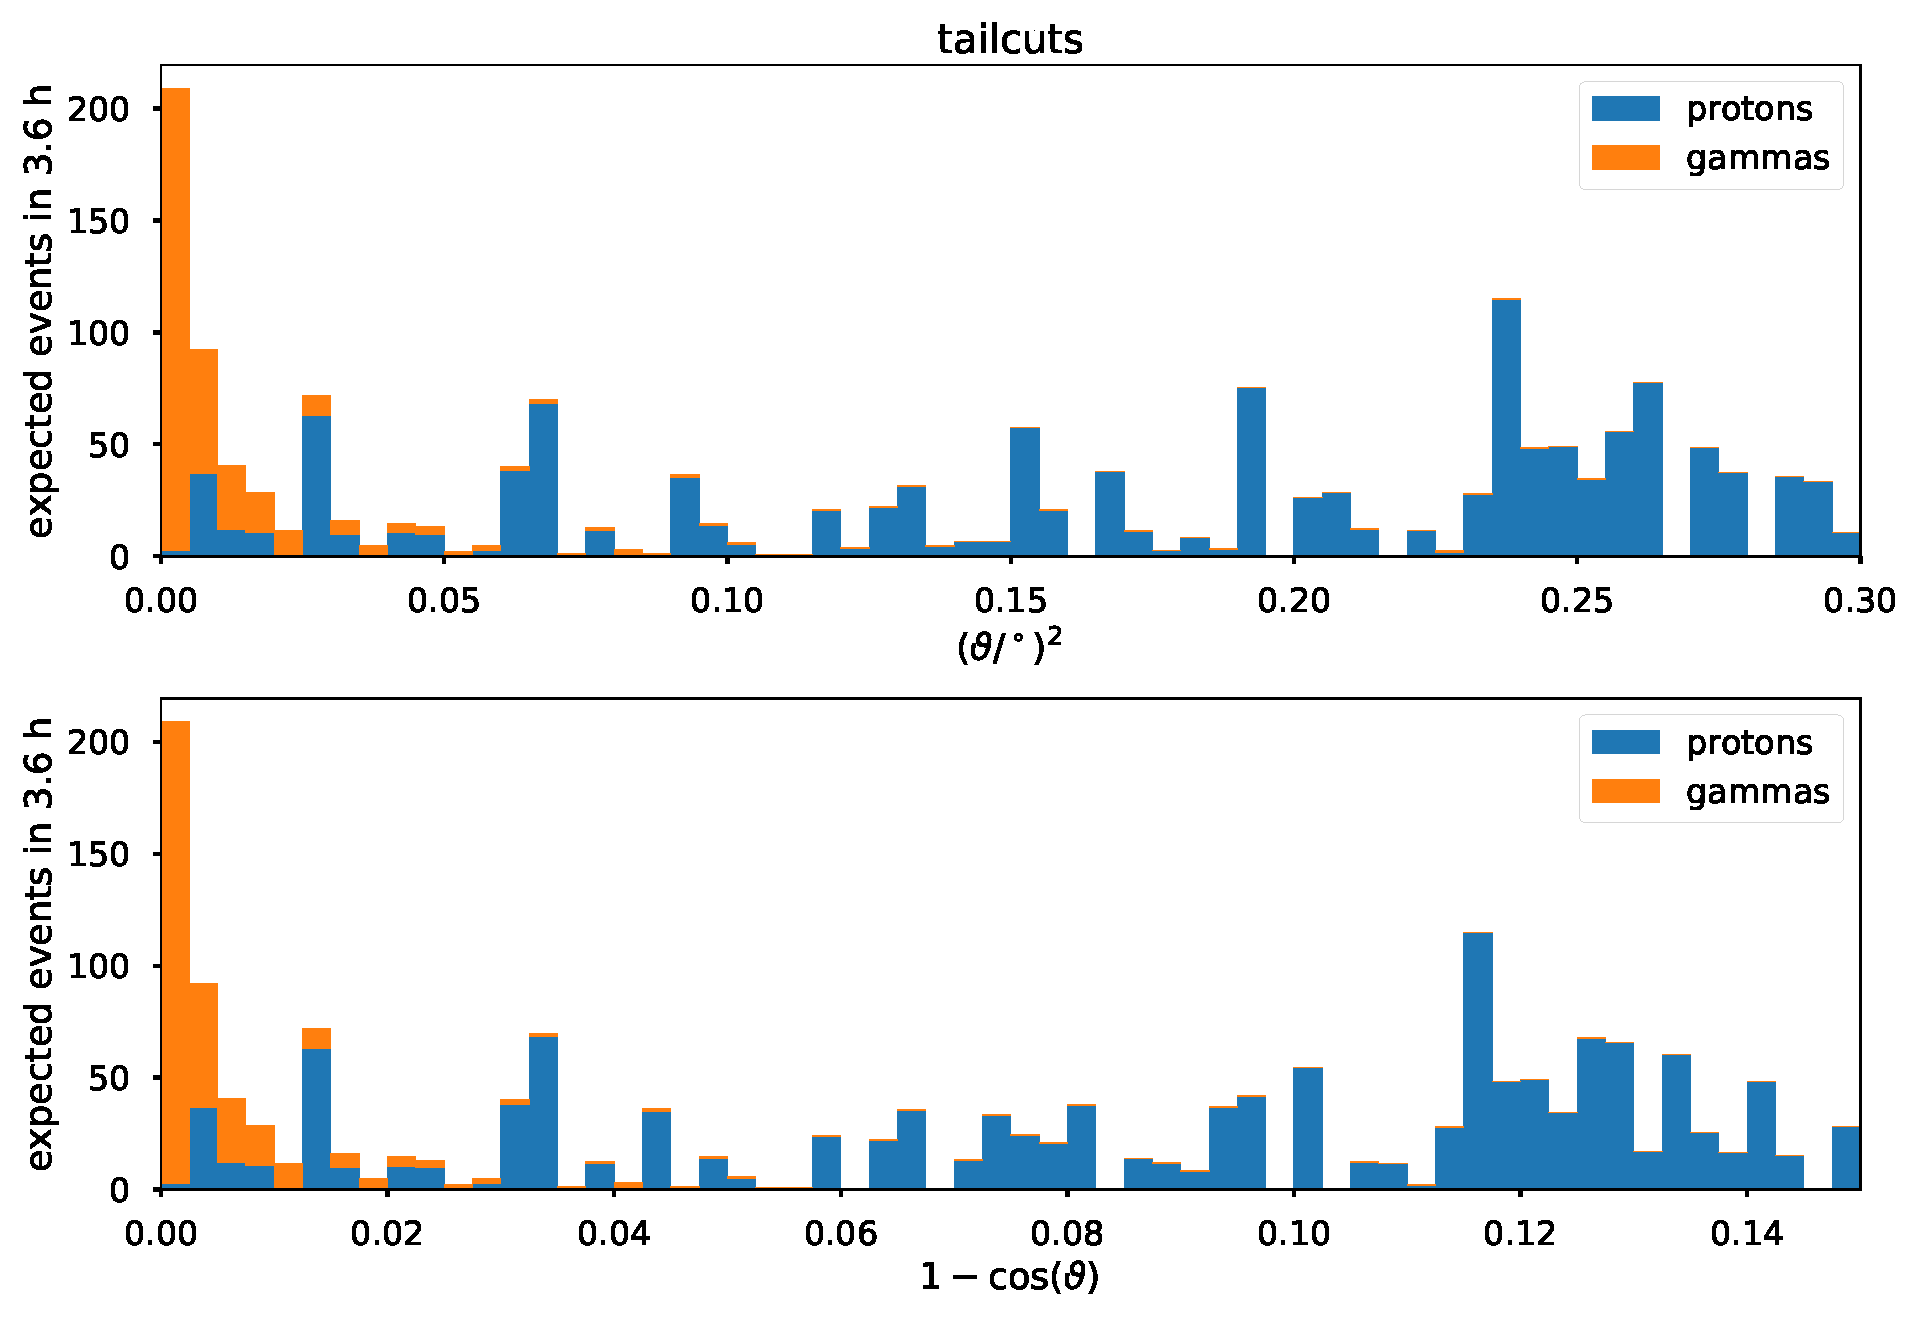
\includegraphics[width=\textwidth]{{pics/theta_square_tail}.pdf}
        }
    \end{frame}


    \begin{frame}[fragile]{calculating Sensitivity}
        \begin{itemize}
            \item define on- and off-regions: \unit{0.15}{\degree} around MC source
            \item[] on-region count $N_\mathrm{on} = N_\gamma + N_\mathrm{p}$
            \item[] off-region count $N_\mathrm{off} = N_\mathrm{p}$
            \item significance given by Li Ma (1983):
            \begin{verbatim}
    alpha1 = alpha + 1.0
    sum    = Non + Noff
    arg1   = Non / sum
    arg2   = Noff / sum
    term1  = Non * np.log((alpha1/alpha)*arg1)
    if Noff == 0:
        term2 = 0
    else:
        term2  = Noff * np.log(alpha1*arg2)
    sigma  = np.sqrt(2.0 * (term1 + term2))
            \end{verbatim}
            \item given the expected $N_\gamma$ from the assumed source, scale the flux up
                or down until $sigma = 5$ \textrightarrow\ this is our sensitivity
        \end{itemize}
    \end{frame}


    \begin{frame}{Sensitivity of the ASTRI mini-array}
        \centering
        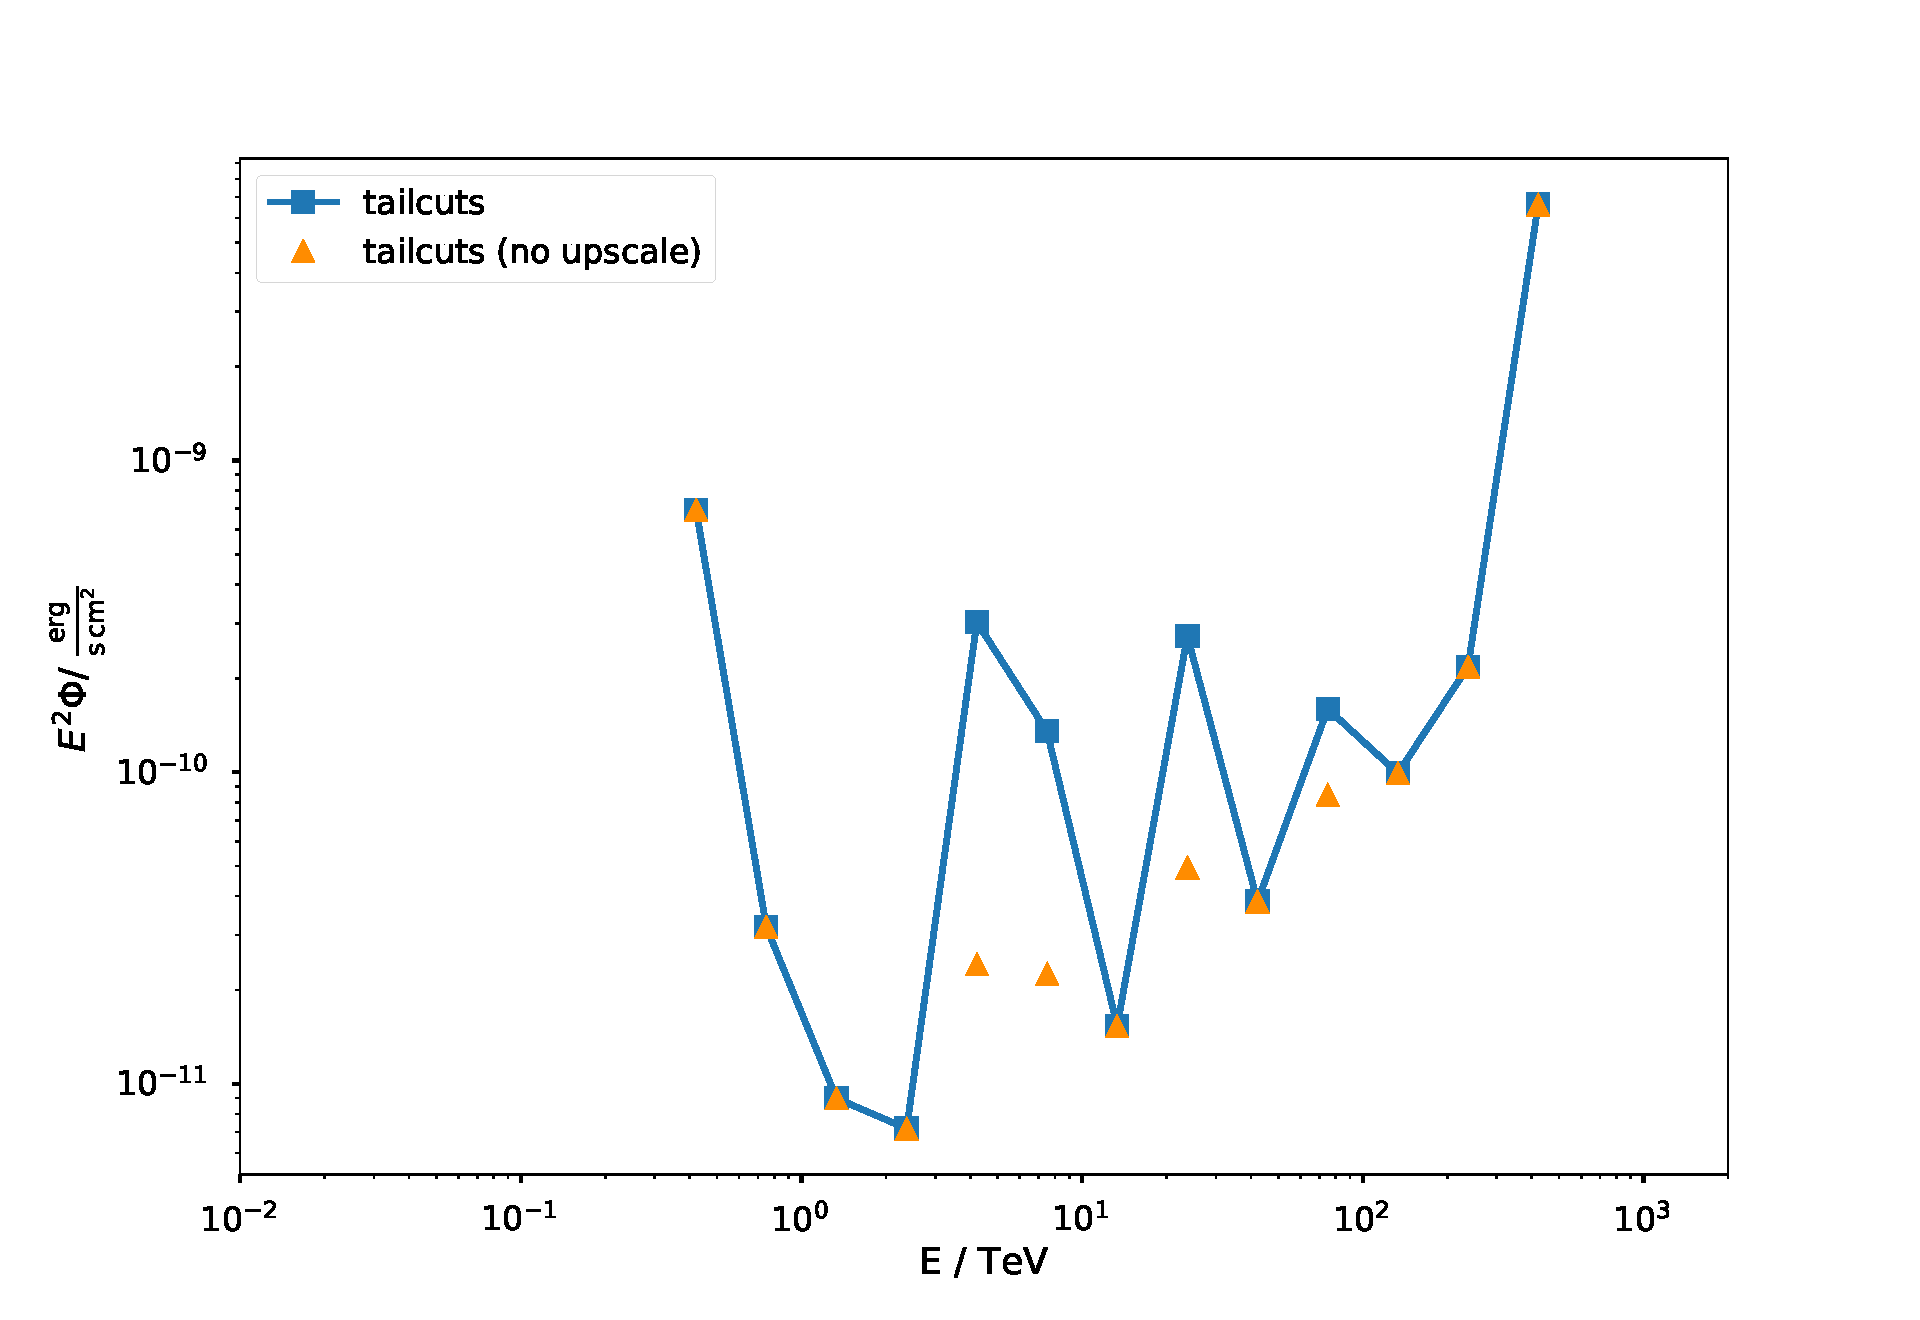
\includegraphics[width=\textwidth]{pics/sensitivity}
    \end{frame}

    \begin{frame}{that blue line...}
        \begin{itemize}
            \item orange triangles represent the $5\sigma$ flux
            \item blue line due to the additional CTA requirements on the sensitivity:
            \item in every energy bin there need to be at least 10 events
            \item and a maximum background contribution of $5\,\%$
        \end{itemize}
    \end{frame}


\end{document}
